% The FYP template is designed according to NTU SCSE FYP guidelines on https://www3.ntu.edu.sg/scse/fyp/UsefulInfo/Report%20Guide.pdf.

% Credit
% Original version by Vincent Ribli
% https://www.overleaf.com/latex/templates/ntu-scse-fyp-template/kwdtcbqmjctk

% Revised by Prof Loy Chen Change
% 23 Aug 2024 - Replace SCSE with CCDS

\documentclass[pdftex, 12pt, a4paper]{report}
\usepackage{newtxtext, newtxmath}
\usepackage[top=3cm, bottom=3cm, left=3.5cm, right=3cm]{geometry}
\usepackage[hidelinks]{hyperref}
\usepackage[pdftex]{graphicx}
\usepackage{booktabs}
\usepackage{setspace}
\usepackage{titlesec}
\usepackage{tocloft}
\usepackage{parskip}
\usepackage{amsmath}
\usepackage{amsfonts}
\usepackage[sorting=none]{biblatex}

\addbibresource{bib.bib}
\setstretch{1.5}
\setlength{\cftfigindent}{0pt}
\setlength{\cfttabindent}{0pt}
\renewcommand{\cftdotsep}{1}

% change the following
\title{\uppercase{Development of Smart Contracts}}
\newcommand\fypcode{SCSE8338}
\author{Harvey Specter}
\date{2024}
\newcommand\degree{Bachelor of Engineering in Computer Science}

\begin{document}
\makeatletter
\begin{titlepage}
\begin{center}

\uppercase{\textbf{\large{Nanyang Technological University}}}
\\[7cm]

\uppercase{\textbf{\large{\@title}}}

\vfill
\@author
\\[3cm]

College of Computing and Data Science

\@date

\end{center}
\end{titlepage}
\makeatother

\makeatletter
\begin{titlepage}
\begin{center}

\uppercase{\textbf{\large{Nanyang Technological University}}}
\\[6cm]

\uppercase{\textbf{\fypcode \\[0.3cm]\@title}}

\vfill

Submitted in Partial Fulfilment of the Requirements\\
for the Degree of \degree\\
of the Nanyang Technological University
\\[0.8cm]
by
\\[0.8cm]

\@author
\\[2cm]

\end{center}

College of Computing and Data Science\\
\@date
\end{titlepage}
\makeatother


\setcounter{page}{1}
\pagenumbering{roman}

\chapter*{Abstract}
\addcontentsline{toc}{chapter}{Abstract}

Lorem ipsum dolor sit amet, consectetur adipiscing elit. Morbi lobortis id nunc a maximus. Nam vitae pellentesque elit. Ut lacus arcu, consectetur at erat sed, sollicitudin suscipit dolor. Sed pharetra, ipsum id volutpat dictum, lacus ante hendrerit mauris, ac tristique orci dui quis dolor. Suspendisse dictum magna vitae fermentum maximus. Quisque vulputate urna id turpis pulvinar suscipit. Praesent sit amet finibus ante. Nullam dignissim sapien ac dolor elementum accumsan. In fermentum tellus eu velit ullamcorper pellentesque id eu eros. Phasellus erat elit, luctus eleifend urna eu, consequat fringilla nisl. Aenean convallis mattis libero, eu dignissim ligula mollis at. Cras pharetra imperdiet risus, in placerat sem ultrices ultrices. Donec eget augue condimentum, efficitur nunc vel, fermentum lacus.

\chapter*{Acknowledgments}
\addcontentsline{toc}{chapter}{Acknowledgments}

The writer uses this section to thank all those he or she is indebted for guidance, financial or any other assistance rendered during the course of the project.




\pagebreak
\addcontentsline{toc}{chapter}{Contents}
\tableofcontents

\pagebreak
\addcontentsline{toc}{chapter}{List of Tables}
\listoftables

\pagebreak
\addcontentsline{toc}{chapter}{List of Figures}
\listoffigures

\cleardoublepage
\pagenumbering{arabic}

\chapter{Introduction}

\section{Background}

\subsubsection{Motivation}

Lorem ipsum dolor sit amet, consectetur adipiscing elit. Morbi lobortis id nunc a maximus. Nam vitae pellentesque elit. Ut lacus arcu, consectetur at erat sed, sollicitudin suscipit dolor. Sed pharetra, ipsum id volutpat dictum, lacus ante hendrerit mauris, ac tristique orci dui quis dolor. Suspendisse dictum magna vitae fermentum maximus. Quisque vulputate urna id turpis pulvinar suscipit. Praesent sit amet finibus ante. Nullam dignissim sapien ac dolor elementum accumsan. In fermentum tellus eu velit ullamcorper pellentesque id eu eros. Phasellus erat elit, luctus eleifend urna eu, consequat fringilla nisl. Aenean convallis mattis libero, eu dignissim ligula mollis at. Cras pharetra imperdiet risus, in placerat sem ultrices ultrices. Donec eget augue condimentum, efficitur nunc vel, fermentum lacus \cite{book}.

\begin{table}[!ht]
    \centering
    \begin{tabular}{@{}cc@{}}
    \toprule
    Cast            & Actor / Actress \\ \midrule
    Harvey Specter  & Gabriel Macht   \\
    Mike Ross       & Patrick J Adams \\
    Jessica Pearson & Gina Torres     \\ \bottomrule
    \end{tabular}
    \caption{Casts}
\end{table}

\begin{figure}[!ht]
    \centering
    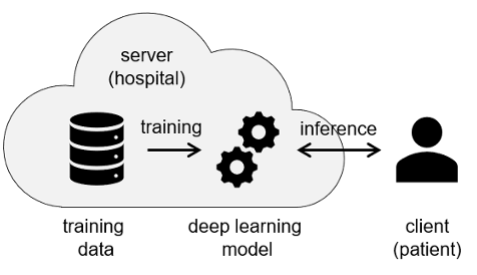
\includegraphics{figures/diag.png}
    \caption{Image}
\end{figure}



\printbibliography

\end{document}
